\chapter{Utility Usage Examples}\label{c:examples}

Examples of the usage of the utilities described in the report will be
given in this chapter.  A two-dimensional finite element model of a
portion of a transportation container will be used for most of the
examples.  The outline of the model is shown in Figure~\ref{exmodel}.
\begin{figure}
\centering
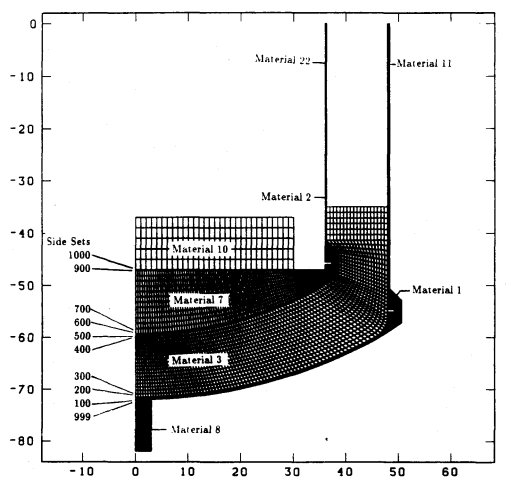
\includegraphics[scale=0.75]{figures/Model.png}
\caption{Finite Element Model for \numbers\ Examples}\label{exmodel}
\end{figure}
The model is composed of nine materials.  Material~1 is the outer shell
which is a $\sfrac{3}{8}$-inch thick stainless steel wall with four
elements through the thickness.  Material~2 is the inner shell which is
a $\sfrac{1}{4}$-inch thick stainless steel wall with three elements
through the thickness.  The energy-absorbing foam between the inner and
outer shells is Material~3.  Above the inner shell is another layer of
energy-absorbing foam which is Material~7;  on top of the foam is a thin
0.120-inch thick steel sheet (Material~9), and the cargo material
(Material~10).  Materials 11 and~22 are the same thickness as Materials
1 and~2, respectively, except that the density has been increased to
account for the top half of the container.  The 6-inch diameter punch at
the bottom of the model is Material~8.  There are five contact surfaces
in this model that are defined by ten side sets.  The contact surfaces
and the corresponding side set identifications and locations are defined
in the following table.

\begin{center}
\begin{tabular}{|ccl|}\hline
Contact  & Side Set  &  Location \\
Surface  & Number    &            \\ \hline \hline
      1  &  100      &  Bottom of outer shell \\
         &  999      &  Top and side of punch      \\ \hline
      2  &  200      &  Top of outer shell    \\
         &  300      &  Bottom of energy-absorbing foam  \\ \hline
      3  &  400      &  Top of energy-absorbing foam  \\
         &  500      &  Bottom of inner shell         \\ \hline
      4  &  600      &  Top of inner shell \\
         &  700      &  Bottom of foam beneath cargo  \\ \hline
      5  &  900      &  Top of sheet beneath cargo \\
         & 1000      &  Bottom of cargo   \\ \hline
\end{tabular}
\end{center}

Several of the utilities in \numbers\ were used during the development
of this model.  Examples of the \cmd{mass properties}, \cmd{overlap},
\cmd{locate}, and \cmd{timestep} utilities will be shown below using the
above model.

\section{\cmd{mass properties} Utility Example}
The \cmd{mass properties} command was used to determine the
pseudo-densities of Materials 10, 11, and~22.  These densities are
called ``pseudo-densities'' since the density is modified to account for
the mass of the body that was omitted from the finite element model.
Material~10 is the cargo material that has a total mass of 22.0~lb-s$^2$/in
(8,500~pounds), and Materials 11 and~22 are the tops of the inner and
outer shells which are used to simulate the mass of the top half of the
container.  The \cmd{mass} utility was used to determine the volume of
each of the materials in the model.  The density of the cargo
(Material~10) was then calculated by dividing the cargo mass by the
cargo volume.  Materials 11 and~22 are intended to simulate the mass of
the upper half of the container.  The density $\rho_{11}$ of Material~11
is calculated as:
\begin{equation}
\rho_{11} = \rho_1 (V_1 + 2V_{11}) / V_{11}
\end{equation}
where $\rho_1$ and $V_1$ are the density and volume of Material~1, and
$V_{11}$ is the volume of Material~11.  The input required to calculate
the mass properties for an axisymmetric body with distinct densities
using four-point quadrature is:

\begin{verbatim}
      AXISYMMETRIC
      DENSITY
      7.324E-04  OUTER_SHELL
      3.297E-03  MASS_OUTER_SHELL
      1.035E-05  FOAM
      7.324E-04  INNER_SHELL
      2.901E-03  MASS_INNER_SHELL
      1.603E-05  CARGO_FOAM
      7.324E-04  PUNCH
      7.324E-04  THIN_SHEET
      7.781E-04  CARGO_MASS
      MASS 4
      EXIT
\end{verbatim}

Figure~\ref{exmassout} shows the resulting output.  Note that the
material labels cannot contain spaces; the character ``\_'' was used to
simulate a space. Although only the masses and volumes were needed for
this example, the output also shows the location of the centroid, the
mass moments of inertia, and the minimum, maximum, and average element
volumes for each material block.

The mass properties utility was also used during the documentation of
this analysis to estimate the weight savings due to using a thinner
wall.  A separate analysis of this body was performed with a
\sfrac{3}{8}-inch thick inner wall and a \sfrac{1}{2}-inch thick outer wall.
\numbers\ was then run to determine the mass of the inner and outer
shells for both models so that the weight differences could be
calculated.

\begin{figure}
\verbatiminput{mass_example_out}
\caption{Output for Mass Properties Example}\label{exmassout}
\end{figure}

\section{\cmd{overlap} Utility Example}
This example will show the input and output for the \cmd{overlap}
utility.  Each of the contact surfaces in the model will be checked to
see if they are penetrated.  Since this is a model that has already been
tested, none of the contact surfaces overlap.
The input for the command is:

\begin{verbatim}
      OVERLAP  100   999
      OVERLAP  200   300
      OVERLAP  400   500
      OVERLAP  600   700
      OVERLAP  900  1000
      EXIT
\end{verbatim}

where the first flag is the master surface and the second flag is the
slave surface. Figure~\ref{exoverlapout} shows the resulting output.
Normally, the contact surfaces should be checked in both directions,
that is, check first with one flag as the master and then check again
with that flag as the slave.  Figure~\ref{exoverlap2} shows the output
from the overlap utility when the contact surfaces do overlap.  The
output shows the number of the penetrating node, the number of the
penetrated element, and the connectivity of the element.

\begin{figure}
\verbatiminput{overlap_example_out}
\caption{Output for Overlap Utility Example--No
Penetration}\label{exoverlapout}
\end{figure}

\begin{figure}
\verbatiminput{overlap2_out}
\caption{Output for Overlap Utility
Example--Penetration}\label{exoverlap2}
\end{figure}

\section{\cmd{locate} Utility Example}

The analysis performed on the example finite element model was concerned
with the response of the outer steel shell due to the impact with the
punch.  The relatively thin outer shell of this model makes it very
difficult to examine the results of the finite element analysis since it
is not possible to plot contours of the stresses or strains in the steel
shell.  However, the \code{SPLOT} module in the postprocessing code
\code{BLOT}~\cite{BLOT} can be used to plot the stresses and strains as
a function of the element number.  Although it is possible to determine
the element numbers of the elements in the outer shell by looking at
plots of the model, an easier and more efficient method is to use the
\cmd{locate} command.  The outer shell has a inner radius of
95.75~inches and a thickness of \sfrac{3}{8}~inch.  Since there are four
elements through the thickness, each element is \sfrac{3}{32}~inch thick.
Using the \cmd{locate point} command with the center point at the center
of curvature (0.0, 24.2) and a distance of 95.75 + \sfrac{3}{64}\ will
locate all elements in the innermost element row; a distance of 95.75 +
\sfrac{21}{64} will locate all elements in the outermost element row.
The input used to locate all elements in the outermost element row is:

\begin{verbatim}
      SORT THETA
      LOCATE ELEMENTS POINT   0  24.2     96.078125   .001
      EXIT
\end{verbatim}

Figure~\ref{exlocateout} is the resulting output.  The output is sorted
on the \cmd{theta} field so that the elements are ordered from the
centerline outward.

\begin{figure}
\verbatiminput{locate_example_out}
\caption{Output for Locate Utility Example--No Penetration}\label{exlocateout}
\end{figure}

\section{\cmd{limits} Utility Example}
The \cmd{limits} utility is executed simply by entering the command {\tt
LIMITS}.  The resulting output is shown in Figure~\ref{exlimitsout}.

\begin{figure}
\verbatiminput{limits_example_out}
\caption{Output for Limits Utility Example}\label{exlimitsout}
\end{figure}

\section{\cmd{timestep} Estimation Example}

The final example using this model will be the estimation of the
timestep using the \cmd{timestep} command.  The input is:

\begin{verbatim}
      WAVESPEED
      2.273e+05  OUTER_SHELL
      1.071e+05  MASS_OUTER_SHELL
      2.003e+04  FOAM
      2.273e+05  INNER_SHELL
      1.142e+05  MASS_INNER_SHELL
      2.731e+04  CARGO_FOAM
      2.273e+05  PUNCH
      2.273e+05  THIN_SHEET
      1.525e+05  CARGO_MASS
      TIMESTEP
      EXIT
\end{verbatim}

The resulting output is shown in Figure~\ref{extimestepout}.

\begin{figure}
\verbatiminput{timestep_example_out}
\caption{Output for Timestep Estimation Utility
Example}\label{extimestepout}
\end{figure}
The minimum timestep is 2.273$\times 10^{-7}$ seconds for Material~2 (the inner
shell).  This is exactly equal to the timestep that was used in
the \code{PRONTO2D} analysis.  For this problem, the average CPU time
per element per timestep in \code{PRONTO2D} was 13.3~$\mu s$.  Since
there are 6,825 elements and 4,399 timesteps per millisecond of analysis
time, the estimated CPU time per millisecond is 400~seconds.  The actual
CPU time per millisecond was 395~seconds.  This example shows that it is
possible to get a very accurate estimate of the time required to perform
an analysis prior to running the analysis.  The timestep estimation is
also useful in determining which material has the smallest or
controlling timestep; if the material with the controlling timestep is
not in the area of interest, reducing the refinement in that material
will give a larger timestep and less analysis time.
